\chapter{Hidden Markov Models}
\label{CHAPTER:HMM}

\abbreviation{Hidden Markov Models}{HMM} are graphical probabilistic models
commonly used to sequence annotation or sequence alignment. An HMM is
a probabilistic finite state machine that in every state emits one symbol. Later
we will also discuss variants of HMMs that emit more symbols or that emit symbols on multiple
tapes. In this chapter, we will describe basic
definitions and algorithms that are used with HMMs.

\section{Definitions}\label{SECTION:HMMDEF}
                       
%HMM
%Pravdepodobnost
%Posterior pravdepodobnost
%Anotacia
%Pravdepodobnost anotacie
%Footprint
HMMs are generative probabilistic models.
The generative process of an HMM starts in a random state $q$ sampled according
to the \firstUseOf{initial
distribution} $I$.  When an HMM is in some state $q$ it emits one symbol from
alphabet $\Sigma$ according distribution $e_q$ and moves to another state
according to transition distribution $a_q$. Note that emission and transition
distributions can be different for every state.  This process produces two
sequences: sequence of states $\pi=\pi_0\pi_1\pi_2\dots$ called
\firstUseOf{state path} and output sequence $X=X_0X_1X_2\dots$ over alphabet
$\Sigma$. In this work we will use only discrete versions of HMMs with finite state
space and alphabet.  


\begin{definition}
Any square matrix $M$ of size $n\times n$ is \firstUseOf{stochastic} if satisfy
following properties.
\begin{enumerate}
\item $\forall 0\leq i<n,0\leq j < m, 0\leq M[i,j]\leq 1$
\item $\forall 0\le i<n, \sum_{i=0}^{m-1}M[i,j]=1$
\end{enumerate}
\end{definition}

\begin{note}
Stochastic matrix consists from $n$ distributions over set of size $n$.
\end{note}

\begin{definition}\label{DEF:HMM}
A \abbreviation{Hidden Markov Model}{HMM} is a tuple $H=(\Sigma,V,I,e,a)$ where
$\Sigma=\{\sigma_0,\dots\sigma_{m-1}\}$ is a finite alphabet of size $m$,
$V=\{v_0,\dots,v_{k-1}\}$ is a finite set of state of size $k$, $I$ is
a distribution over $V$, $e$ is $k\times m$ matrix where each row contains
distribution over $\Sigma$ and $a$ is stochastic matrix of size $m\times m$.

We will index elements of $e$ and $a$ by subscripts, therefore $e_{u,v}$ is
element in $u$-th row and $v$-th column of $e$.  

%Therefore following conditions hold:
%\begin{enumerate}
%\item $\forall v\in V, I_v \geq 0$
%\item $\sum_{v\in V}I_v=1$
%\item $\forall u\in V,\forall \sigma\in\Sigma, e_{u,\sigma}\geq0$
%\item $\forall u\in V, \sum_{\sigma\in \Sigma}e_{u,\sigma}=1$
%\item $\forall u,v\in V, a_{u,v}\geq0$
%\item $\forall u\in V, \sum_{v\in V}a_{u,v}=1$
%\end{enumerate}
\end{definition}

\begin{example}\label{EXAMPLE:EXAMPLEHMM} Consider the HMM $H=(\Sigma,V,I,e,a)$ from figure
\ref{FIGURE:EXAMPLEHMM}.  Alphabet is $\Sigma=\{A,C,G,T\}$ and set of states is
$V=\{R,In,E\}$.  Transition and emission distributions are described in the figure.
We can define initial distribution to $I_R=0.5, I_E=0.3$ and $I_{In}=0.2$.

%Let $H=(\Sigma,V,I,e,a)$ be an HMM with
%$\Sigma=\{A,C,G,T\}$, $V={I,G}$, $I=(0.2,0.8)$,
%$e_{I,A}=0.1,e_{I,C}=0.2,e_{I,G}=0.3,e_{I,T}=0.4, e_{G,x}=0.25, x\in \Sigma$ and 
%$a_{I,I}=0.9,a_{I,G}=0.1,a_{G,G}=0.95$ and $a_{G,I}=0.05$.
\end{example}

%The conditions $1-6$ ensure that everything is correct probabilistic
%distribution.
\begin{figure}
\begin{center}
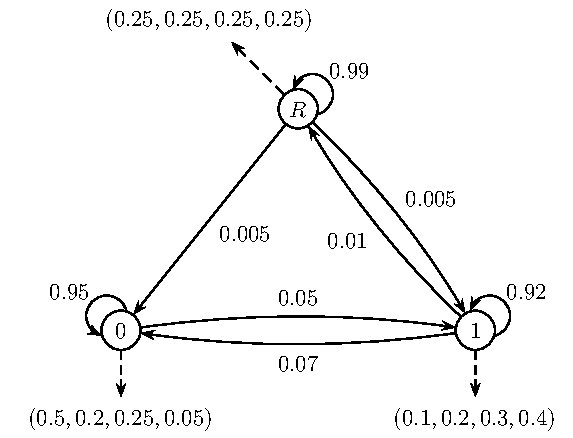
\includegraphics{../figures/exampleHMM.pdf}
\end{center}
\caption[Example of simple Hidden Markov Model]{
A HMM with $3$ states
that emits symbols from alphabet of size $4$.  Circles represents states, arc
from state $u$ to $v$ indicated that $a_{u,v}>0$. Missing arc from state
$In$ to $R$ means that $a_{In,R}=0$.  There are also arcs between states and
four tuples. Everu four tuple represents emission distribution of associated state.
}\label{FIGURE:EXAMPLEHMM} 
\end{figure}


\begin{definition}\label{DEF:STATEPATH}
Let $H=(\Sigma,V,I,e,a)$ be an HMM. We say that there is \firstUseOf{transition}
from state $u$ to state $v$ if $a_{u,v}>0$. We will write transition from $u$ to
$v$ as $u\to v$ and $T=\{u\to v\mid a_{u,v}>0\}$ is set of all transitions of
$H$.

\firstUseOf{State path} $\pi=\pi_0\pi_1\dots\pi_{n-1}$ is a sequence of
states. We say that state path $\pi$ is \firstUseOf{admissible} if $I_{\pi_0}>0$
and  $\pi_{i-1}\to\pi_i\in T$ for all $1\leq i < n$. Otherwise $\pi$ is
\firstUseOf{inadmissible}.
\end{definition}

\begin{example}
Consider HMM from figure \ref{FIGURE:EXAMPLEHMM}. Set of transitions is
$T=\{R\to R,R\to In, R\to E,In\to In, In\to E, E\to E, E\to In, E\to R\}$.
State path $\pi_1=RRRRInER$ is admissible state path and $\pi_2=RRRInREER$ is inadmissible
state path, because contain transition with zero probability ($In\to R$).
\end{example}



%Formally, Hidden Markov Model is defined by it's finite state space
%$Q=\{q_0,q_2,\dots, q_{k-1}\}$ of size $k$, initial probabilistic distribution
%$I$ over state space, finite alphabet $\Sigma = (\sigma_0, \sigma_1, \dots,
%\sigma_{m-1})$ of
%size $m$, emission and transition distribution over $\Sigma$ and $Q$
%respectively defined for every state independently. We denote emission
%distribution of state $q$ by $e_q$ and transition distribution by $a_{q}$. 

Since Hidden Markov Models are generative probabilistic models, we have to
define probability distribution of HMM's products. In following definitions we
will define probability distribution of pairs (state path, sequence) and
probability distribution of sequences generated by an HMM.

\begin{definition}
Let $H=(\Sigma,V,I,e,a)$ be an HMM and $X=X_0X_1\dots X_{n-1}$ be a sequence over
alphabet $\Sigma$ of length $n$. Let $\pi$ be a state path of length $n$. Then the
probability that state path $\pi$ generated sequence $X$ is 

\[\prob{X,\pi\mid H}=
I_{\pi_0}e_{\pi_0,X_0}\prod_{i=1}^{|X|-1}a_{\pi_{i-1},\pi_i}e_{\pi_i,X_i}\]

If length of the sequence $X$ is not equal to length of the state path $\pi$,
then
probability that $\pi$ generates $X$ is zero.
\end{definition}



\begin{example}
Consider HMM $H$ from example \ref{EXAMPLE:EXAMPLEHMM}. Let state path be $\pi=RRInInE$ and
generated sequence be $X=ACGTT$. Then the probability that $H$ generates $\pi$
and $X$ is 
$\prob{ X,\pi\mid H } = 0.5 \cdot 0.35 \cdot 0.99 \cdot 0.25 \cdot 0.005 \cdot 0.25 \cdot 0.95 \cdot 0.05 \cdot 0.05 \cdot 0.4 =
0.5143359375  \cdot  10^{-7}$
\end{example}

\begin{definition}
Let $H=(\Sigma,V,I,e,a)$ be a HMM and $X=X_0X_1\dots,X_{n-1}$ be a sequence over
alphabet $\Sigma$ of length $n$. The probability that $X$ was generated by the
model $H$ is 
\[\Pr\left(X\mid H\right)=\sum_{\pi\in V^n}\Pr\left(X,\pi\mid H\right)\]
\end{definition}



\begin{note}
In our  definition of an HMM, the sum of the probabilities of all sequences of
length $n$ is $1$. Later we will discuss concept of final states. With final
states, the sum of the probabilities of all sequences (of all lengths) is one.

\end{note}

We will be interested in the three basic problems in HMMs:
\begin{enumerate}
\item Given sequence $X$ and model $H$. What is the probability that $X$ was
generated by model $H$?
\item Given sequence $X$, model $H$ and assumption that $X$ was generated by the
model
$H$, what is the best explanation of $X$? By explanation is usually meant state
path that generated $X$. We call the process of computing explanation of
sequence $X$ \firstUseOf{decoding}.
\item Given training data $D$ (usually sequences with ``explanations'') and
topology of model (set of states and transitions), what are the best parameters
(initial, transition and emission distributions) that explains train
data $D$? This problem is also called \firstUseOf{training}
\end{enumerate} 
In following sections we will discuss several algorithms
that are trying to solve problems describes above. We will mostly focus on the
decoding problem.


\section{The Forward Algorithm}
The Forward algorithm \cite{Durbin1998} computes for a given sequence $X$ of
length $n$ the probability $\Pr\left(X\mid H\right)$ that sequence was
generated by the model (it solves the first problem of HMM). The algorithm is
based on the dynamic programming. It fills
matrix $F$ of size $n\times m$ where $F[i,v]$ is the probability that $H$
generated $X[:i+1]$ with state path that ends in state $v$ and $m$ is the number
of states of $H$. Values $F[i,v]$ are  called \firstUseOf{forward
variables}. $F[i,v]$ can be computed by following equations (also called the
forward equations).

\begin{align}
F[0,v] &= I_ve_{v,X_0}, v\in V\\
F[i,v] &= \sum_{u\in V}F[i-1,u] \cdot a_{u,v} \cdot e_{v,X_i}, v\in V,0< i < n
\end{align}
%We call values $F[i,v]$ forward variables. Value $F[i,v]$ is the
%probability, that $X[:i+1]$ was generated by state path that ends with state
%$v$. 
The probability that $H$ generated $X$ is 
 \[\Pr\left(X\mid H\right) = \sum_{v\in V} F[|X|-1,v]\]

Using the recurrence equations above, we can compute the probability of $X$ in
$O(nm^2)$ time and $O(m)$ memory dynamic programming where $n$ is the length
of the input sequence and $m$ is the number of states of $H$. If the transition
matrix is sparse, then this algorithm can be implemented in $O(n(m+t))$ time
where $t$ is the number of transitions.  Forward variables are also used in other
algorithms. 
%Storing all of the forward variables requires soring $O(nm)$ numbers.

\section{Sequence Annotation}

%definujeme annotation, footprint, set of colors

HMMs can be used for sequence annotation. By sequence annotation we mean
assigning ``labels'' to parts of the input sequence according to their meaning.
Now we give few examples.

\paragraph{Gen e finding:} in cells parts of DNA sequences that are translated
into proteins are called genes.  In gene finding we want to assign to every
symbol of input sequence gene label if it is inside gene (and optionally exon
or intron label) and other label is that symbol is not part of a gene
\cite{GeneWise2004,Brejova2005,Burge1997,Alexanderson2004}.

%For example in the gene-finding domain, we want to assign gene labels to those
%parts of the sequence that encode proteins. To annotate transmembrane proteins,
%we want to know, which parts of the sequence are on which  side of the membrane.
%In recombination prediction we want to predict which parts of the sequence
%belong to which subtype of an organism.  \todo{rozviest priklady, alebo zrusit}

\paragraph{Transmembrane proteins:} some proteins in cells pass through membrane
from one side to the another (usually they pass membrane several times).  In
transmembrane protein prediction we want to assign to labels to symbols of input
sequence to distinguish the parts of the sequence that are on one side of a
membrane from the parts that are on the other side of the membrane or that are
inside membrane \cite{Brown2010}.
%input sequence according to the side of the membrane Aim of transmembrane
%proteins is to predict which parts of the protein sequence is on which part of
%membrane and which parts are in membrane.

\paragraph{Recombination prediction:} Some organisms, for example HIV virus,
evolves rapidly and have been classified into several subtypes.  Moreover,
some viruses are mosaic combination of viruses from different subtypes. For
example beginning and end of the RNA sequence of virus can be from one subtype and
the middle of the sequence is from different subtype. In recombination prediction
we want to annotate RNA sequence to distinguish between parts that originate in
different subtypes \cite{Nanasi2010,Truszkowski2011}.  

\paragraph{} In general,
we have a finite set of labels $C=\{c_0,c_1,\dots,c_{l-1}\}$ and we want to
assign one label to every symbol of the input sequence. We do it by assigning
one label to every state of an HMM.
%in a way, that states of HMM that encodes same meaning have same color. After
%that we try 
To predict the annotation of the input sequence $X$, we can  find the
most probable state path that can generated $X$ and  annotate each symbol of
the sequence $X$ according to the label assigned to the state that generated that
symbol. We can formalized it in the following definition.

\todo{Aby nebol bordel medzi label a color}

\begin{definition}\label{DEFINITION:ANNOTATION}
Let $H=(\Sigma,V,I,e,a)$ be HMM and $C=\{c_0,c_1,\dots,c_{l-1}\}$ be the finite
sets of labels (or colors). Then the \firstUseOf{coloring function} 
$\lambda: V^*\to C^*$ is function that satisfies following properties:
\begin{enumerate}
\item $\lambda(v)\in C$ for all $v\in V$.
\item $\lambda(xy) = \lambda(x)\lambda(y)$ for all $x,y\in V^*$.
\end{enumerate}

Let $X$ be sequence generated by state path $\pi$. Then annotation
$\Lambda$ of sequence $X$ is $\Lambda = \lambda(\pi)$.
\end{definition}

In the sequence annotation we do not know the state path $\pi$ that generated a given
sequence. Our goal is to reconstruct the state path $\pi$ or at least to give a good
approximation of the correct annotation $\Lambda(\pi)$. Note that in general, several state
paths can have the same annotation.

%Since many states of the HMM can have assigned same label, there may be may be
%many state path with same annotation.

\begin{definition}
Let $H$ be an $HMM$, $X$ be a sequence of length $n$, $\Lambda$ be an annotation of sequence
$X$. The probability of annotation $\Lambda$ given sequence $X$ is 
\begin{equation}
\Pr\left(\Lambda\mid X,H\right)=\sum_{\pi \in V^n,\lambda(\pi) =
\Lambda}\Pr\left(\pi\mid X,H \right)\label{DEF:ANNOTATION:PROBABILITY}
\end{equation}
\end{definition}

Note that $\prob{\pi\mid X,H}=\frac{\prob{\pi,X\mid H}}{\prob{X\mid
H}}$

\begin{example}\label{EXAMPLE:ANNOTATION}
Let $H$ be the HMM from example \ref{EXAMPLE:EXAMPLEHMM}. Let $C=\{I,G\}$ and
$\lambda(R)=I$ and $\lambda(In)=\lambda(E)=G$.  Then annotation of sequence
$X=AACT$, which was generated by the state path $\pi=RInEE$. The correct
annotation of $X$ is therefore  $\lambda(RInEE) =
IGGG$. 

We will use following interpretation of the model $H$. We can imagine $H$ as very simple gene
predictor\footnote{Not very realistic}. $R$ represents intergenic regions, state $In$
represents introns and $E$ represents exons. Label $I$ represents
intergenic region and label $G$ represents regions that are genes.

Using this interpretation, the sequence $AACT$ contains gene $ACT$. There are
several explanations of this ``fact'': if $AACT$ was generated by state path
$REEE$ then subsequence $EEE$ is exon; if it was generated by state path $REIE$
then sequence contain two exons and one intron in the middle. There are $2^3$
different state paths $\pi$ with $\lambda(\pi)=IGGG$.  All of those state path
support ``fact'' that $IGGG$ is the correct annotation of $X$.

\end{example}


%\begin{example}
%Consider again HMM from example \ref{EXAMPLE:EXAMPLEHMM} and annotation function
%from example \ref{EXAMPLE:ANNOTATION}.
%\end{example}

Given a sequence $X$, the natural question is what is the best annotation of
$X$.  One measure of quality of an annotation is it's probability. The more
probable is annotation, the more likely $X$ was generated with state path with
such annotation. We can formulate this in following problem.

\begin{definition}
Given HMM $H$ and sequence $X$, \abbreviation{the most probable annotation
problem}{MPA} is the problem of finding an annotation of $X$ that maximizes
the probability \[\prob{\Lambda\mid X,H}\]
\end{definition}

\begin{theorem}
Most probable annotation problem is NP-hard.
\end{theorem}
This theorem was proved in 2002 by Lyngsø {\it et al.} and proof can be found in
\cite{Lyngso2002}. Their proof was done by conversion to the maximal clique problem.
For input graph with $n$ vertices they construct an HMM $H$ with $O(n^2)$ states and
sequence $X$ of the length $n$. The most probable annotation of $X$ could be
converted into maximal clique of input graph. 

\begin{theorem}
There exists an HMM such that it is HP-hard to find the most probable annotation
to given sequence $X$.
\end{theorem}
The proof of this theorem can be found in \cite{Brejova2007mpa}. This paper also
contain polynomial algorithm (Extended Viterbi Algorithm) that finds most
probable annotation for special classes of HMMs. 

Note that from the probabilistic nature of the HMMs, the most probable
annotation does not have to be the best approximation of the correct annotation.
Alternative decoding criteria can improve quality of annotations in specific
applications \cite{Brown2010,Gross2007,Nanasi2010,Truszkowski2011}.

\section{The Viterbi Algorithm}
%\todo{Viterbi variable ma rovnake oznacenie ako mnozina stavov. Treba to
%upravit} -- Brona tvrdi ze netreba
The Viterbi algorithm  is probably the most frequently used
decoding algorithm for Hidden Markov
models \cite{Durbin1998}.
The Viterbi algorithm answer a straightforward question: given the sequence
$X=X_0X_1\dots X_{n-1}$, what
is the most-likely state path $\pi$ that generates $X$? Formally, Viterbi
algorithm finds a state path maximizing $\Pr\left( \pi\mid X,H \right)$. Since
\[\Pr\left(\pi\mid X,H\right) = \frac{\Pr\left(\pi,X,\mid
H\right)}{\Pr\left(X\mid H\right)}\] and quantity $\Pr\left(X\mid H\right)$ is
fixed, the most probable state path $\pi$ also maximize $\Pr\left(X,\pi\mid H\right)$. 

The Viterbi algorithm is very similar to the  Forward algorithm. It starts with computing
Viterbi variables $V[i,v]$. Variable $V[i,v]$ stores the probability of the most probable 
state path that generated $X[:i+1]$ and ends in state $v$. The algorithm
also computes back-links $B[i,v]$ that contain the previous state in the most
probable state path that generated $X[:i+1]$ and ends in state $v$. We can
compute these values by the following equations (called the Viterbi equations):
\begin{align}
V[0,v] &= I_{v}e_{v,X_0}, v\in V\\
V[i,v] &= \max_{u\in V} V[i-1,u]a_{u,v}e_{v,X_i}, v\in V,0<i<n\\
B[i,v] &= \arg\max_{u\in V} V[i-1,u]a_{u,v}e_{v,X_i}, v\in V,0<i<n
\end{align}
\begin{note}
Values $B[0,v],v\in V$ are not needed in the algorithm.

Note the similarity of the Viterbi algorithm and the Forward algorithm.
We can obtain the Viterbi equations from the Forward equations by replacing
summation with
maximization.
\end{note}


Variable $V[n-1,v]$ contains the probability of the most probable state path
that generated $X$ and end in state $v$. Therefore the state $v_{\max} =
\arg\max_{v\in V}V[n-1,v]$ is the last state of the most probable state path.
Variable $B[n-1,v_{\max}]$ contains the previous state of the most probable
state path. By traversing back through back-links $B$ we can reconstruct the most
probable state path in $O(n)$ time.

Time complexity of the Viterbi algorithm is $O(nm^2)$ where $m$ is the number of
states. Similarly to the Forward algorithm, if transition matrix is sparse then 
the Viterbi algorithm can be implemented in $O(n(m+t))$ time where $t$ is the
number of transitions of HMM.


We can use the Viterbi algorithm to annotate sequence $X$ by finding the most
probable state path $\pi$ and then computing $\lambda(\pi)$. If the  coloring
function $\lambda$ is the identity function, this will find the most probable
annotation, but in general the Viterbi algorithm is not even a good approximation of
the most probable annotation as shown in the following example.

\begin{figure}
\begin{center}
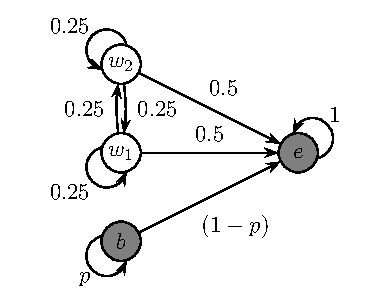
\includegraphics{../figures/multiplePathProblemHMM.pdf}
\end{center}
\caption[Hidden Markov Model with multiple path problem.]{Example of HMM with
multiple path problem. States $w_1,w_2,b$ emits symbol $0$ with probability $1$
and state $e$ emits symbol $1$ with probability $1$. Initial distribution is set
to $I_{w_1}=I_{w_2}=\frac14, I_{b}=0.5$
and $I_e=0$. Annotations of the states are represented by the colors of the states
($\lambda(w_1)=\lambda(w_2)$ and $\lambda(b)=\lambda(e)$. }\label{FIGURE:BADVITERBIEXAMPLE}
\end{figure}

\begin{example}
Consider the HMM from the figure \ref{FIGURE:BADVITERBIEXAMPLE}. Take sequence $X=0^n1$.
Since state $e$ is the only state that can emit $1$, every state path with non-zero
probability ends in state $e$. If state path starts in state $b$ then state
path has form $b^ne$. Annotation of such state path is $\Lambda_1=\lambda(b)^{n+1}$
and probability of the annotation $\Lambda_1$ (and also the state path $b^ne$) is $p^n(1-p)$.
If state path starts in the one of the white states, then the state path
has form $w'_0w'_1\dots w'_{n-1}e$ where $w'_i$ is either $w_1$ or $w_2$.
There are $2^n$ such state paths and each of them have the probability $0.5\cdot
0.25^n$ and annotation $\Lambda_2=\lambda(w_1)\lambda(e)$. Probability of
annotation $\Lambda_2$ is therefore $0.5^{n+1}$.
If $n$ is sufficiently high and $\frac14<p<\frac12$ then most probable state
path is $b^ne$ which corresponds to the annotation $\Lambda_1$. However, the most
probable annotation is $\Lambda_2$ and its probability is exponentially higher
then the probability of $\Lambda_1$. Therefore the Viterbi algorithm it not even a
good approximation of the most probable annotation problem.

We say that an HMM has the \firstUseOf{multiple path problem} if it has an annotation that
corresponds to more than one state path.
\end{example}


\section{The Forward-Backward Algorithm and  the Posterior Decoding}

The \firstUseOf{Posterior decoding} is another commonly used decoding method. In
contrast to the Viterbi algorithm, the Posterior decoding assigns a label individually to
every symbol of an input sequence and does not care about the overall structure of
the reconstructed state path. 

Given sequence $X$, posterior decoding finds state path $\pi$ with the following
property:
\[\forall 0\leq i< n, \pi_i=\arg\max_{v\in V}\Pr\left(\pi_i=v\mid X,H\right) \]
where \[\Pr\left(\pi_i=v\mid X,H\right) = \sum_{\pi\in V^n,\pi_i=v}\Pr\left(\pi\mid X,H\right)\]

Values $\Pr\left(\pi_i=v\mid X,H\right)$ can be computed using the Forward-Backward
algorithm. This algorithm computes $\Pr\left(\pi_i=v\mid X,H\right)$ for every
combination of position $i$ and state $v$. The Posterior decoding choose for
every position the state that maximizes posterior probability.

We derive the formula for efficient computation of the  $\Pr\left(\pi_i=v\mid
X,H\right)$.
\begin{align}
\Pr\left(\pi_i=v,X\mid H\right) &=  
%\sum_{\pi\in V^n,\pi_i=v}\Pr\left(\pi\mid X,H\right)
%					\label{PosteriorDer1} \\
%				&=& 
				\sum_{\pi\in
				V^n,\pi_i=v}I_{\pi_0}e_{\pi_0,X_0}\prod_{j=1}^{n-1}e_{\pi_j,X_j}a_{\pi_{j-1},\pi_j}
					\label{PosteriorDer2}\\
%				&= \sum_{\pi\in V^n,\pi_i=v}I_{\pi_0}e_{\pi_0,X_0}
%				\left( 
%					\prod_{j=1}^{i-1} e_{\pi_j,X_j}a_{\pi_{j-1},\pi_j}
%				\right)
%				a_{\pi_{i-1},\pi_i}e_{\pi_i,X_i}
%				\left(  
%					\prod_{j=i+1}^{n-1} e_{\pi_j,X_j}a_{\pi_{j-1},\pi_j}
%				\right)
%					\label{PosteriorDer3}\\
				&= \sum_{\pi\in V^n,\pi_i=v}I_{\pi_0}e_{\pi_0,X_0}
				\left( 
					\prod_{j=1}^{i-1} e_{\pi_j,X_j}a_{\pi_{j-1},\pi_j}
				\right)
				a_{\pi_{i-1},v}e_{v,X_i}
				\left(  
					\prod_{j=i+1}^{n-1} e_{\pi_j,X_j}a_{\pi_{j-1},\pi_j}
				\right)
					\label{PosteriorDer4}\\
				&= 
				\left(
					\sum_{\pi\in V^{i+1},\pi_i=v}I_{\pi_0}e_{\pi_0,X_0}
					\left(
						\prod_{j=1}^{i} e_{\pi_j,X_j}a_{\pi_{j-1},\pi_j}
					\right)
				\right)
				\left( 
					\sum_{\pi\in V^{n-i},\pi_0=v}
					\prod_{j=1}^{n-i-1} e_{\pi_j,X_{j+i}}a_{\pi_{j-1},\pi_j}
				\right)
					\label{PosteriorDer5}\\
				&= F[i,v]
				\left( 
					\sum_{\pi\in V^{n-i},\pi_0=v}
					\prod_{j=1}^{n-i-1} e_{\pi_j,X_{i+j}}a_{\pi_{j-1},\pi_j}
				\right)
					\label{PosteriorDer6}
\end{align}
The right part of the formula \ref{PosteriorDer6} has
similar structure as $F[i,v]$, but it uses last part of the state path and
sequence and also it lack initial distribution. We can compute 
this formula using  the Backward algorithm, which is very similar to forward
algorithm. Let $B[i,v]$ be the right part of formula \ref{PosteriorDer6}.
\begin{align}
B[i,v]&=
\sum_{\pi\in V^{n-i},\pi_0=v}
	\prod_{j=1}^{n-i-1}
		e_{\pi_j,X_{i+j}}a_{\pi_{j-1},\pi_j}\\
 &= 
 \sum_{u\in V}
 	e_{u,X_{I+1}}A_{V,u}
	\sum_{\pi\in V^{n-i-1},\pi_0=u}
		\prod_{j=1}^{n-i-2}
			e_{\pi_j,X_{i+j+1}}a_{\pi_{j-1},\pi_j}\\
 &= 
 \sum_{u\in V}
 	e_{\pi_j,X_{i+1}}a_{v,u}B[i+1,u]
\end{align}
If we set $B[n-1,v]$ to $1$, we have a recurrence to compute values
$B[i,v]$. This recurrence is very similar to recurrence $F[i,b]$. Recall that
\[F[i,v] = \sum_{u\in V}F[i-1,u] a_{u,v} e_{v,X_i}\]
The cell $B[i,v]$ depends on the next positions in sequence $X$,
while $F[i,v]$ depends on the previous positions in sequence $X$. Another
difference is that $B[i,v]$ does include emission of $X[i]$ while $F[i,v]$ does.

In addition, it is possible to compute probability
of $X$ being generated by the model with backward algorithm.

\begin{align}
\prob{X\mid H} &= 
	\sum_{\pi\in V^n}
		e_{\pi_0,X_0}\prod_{i=1}^{n-1}e_{\pi_i,X_i}a_{\pi_{i-1},\pi_i}\\
	&=
	\sum_{u\in V}e_{u,X_0}
	\sum_{\pi\in V^n,\pi_0=u}
		\prod_{i=1}^{n-1}e_{\pi_i,X_i}a_{\pi_{i-1},\pi_i}\\
	&=
	\sum_{u\in V}e_{u,X_0}B[0,u]
\end{align}

Posterior probabilities can be computed by
\[\Pr\left(\pi_i=v\mid X,H\right) = \frac{F[i,v]\cdot B[i,v]}{\Pr\left( X\mid H
 \right)}\]


We can compute values of $F[i,v]$ and $B[i,v]$ in $O(nm^2)$ time and $O(nm)$
memory. Again, in case of sparse transition matrix, this algorithm can be
altered to run in $O(n(m+t))$ time where $t$ is the number of transitions. We
will discuss possible algorithmic improvements of this algorithm later.

One drawback of an  posterior decoding is that it can reconstruct inadmissible
state path. One example is given below.

\begin{figure}
\begin{center}
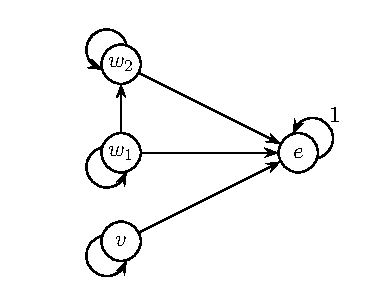
\includegraphics{../figures/posteriorInadmissibleStatePath.pdf}
\end{center}
\caption[Hidden Markov Model on which posterior decoding reconstructs
inadmissible state path]{
Example of an HMM on which the Posterior decoding reconstructs inadmissible state path. 
All unlabeled transitions are even ($0.5$). States $w_1,w_2,$ and $v$ emits $0$
with probability $1$ and state $e$ emits $1$ with probability $1$.
Initial distribution is set to $I_{w_1}=I_{w_2}=0.3, I_{v}=0.4, I_{e}=0$.
}\label{FIGURE:INADMISSIBLESTATEPATH}
\end{figure}

%\todo{Je mozne, ze by sa TU mohlo spomenut a maximalizacii ocakavaneho poctu
%spravne predikovanych stavov}

\begin{example}
Consider an HMM from figure \ref{FIGURE:INADMISSIBLESTATEPATH}. Let $X=001$. There
are three state paths that have non-zero probability:
$\pi_1=w_1w_2e,\pi_2=w_2w_1e$ and $\pi_3=vve$. Their probabilities are
$\prob{\pi_1\mid X,H}=\prob{\pi_2\mid X,H}=0.3, \prob{\pi_3\mid X,H}=0.4$.
Posterior probabilities are in table \ref{TABLE:INADMISSIBLESTATEPATH}.
As we can see, maximal posterior probability for the first position have state
$v$. For the second position it is state $w_2$ and for the third it is state
$e$. Therefore PD will reconstruct state path $vw_2e$. However, this state path 
is inadmissible since  $v\to w_2$ is not a transition (it has zero probability).

\begin{table}
\begin{center}
\begin{tabular}{|l|c|c|c|}
\hline
State/Position & $X_0$ & $X_1$ & $X_2$ \\\hline
$w_1$ & $0.3$ & $0$ & $0$ \\\hline
$w_2$ & $0.3$ & $0.6$ & $0$ \\\hline
$v$   & $0.4$ & $0.4$ & $0$\\\hline
$e$  & $0$ & $0$ & $1$ \\\hline
\end{tabular}
\end{center}
\caption[Example of posterior probabilities.]{Posterior probabilities for
the sequence $X$ and the HMM $H$ from the figure \ref{FIGURE:INADMISSIBLESTATEPATH}.
}\label{TABLE:INADMISSIBLESTATEPATH}
\end{table}

\end{example}


\section{Training} 

Training is the process of estimating parameters of the probabilistic models. In this
section we briefly describe several approaches how to estimate transition and
emission distributions of the hidden Markov models.

We use the \firstUseOf{maximal likelihood approach}. Let $H_{\theta}$ be an HMM
where $\theta$ is vector containing emission and transition probabilities and
$D$ be the training data (sequences with state paths).  We
want to find $\theta$ that maximizes the likelihood of the data:

\[L(H_\theta\mid D)=\prob{D\mid H_\theta}\]

where $D$ is the set of pairs $(X,\pi)$ where $X$ is sequence and $\pi\in
V$. Probability that data
were generated is
\[
\prob{D\mid H_\theta} = \prod_{(X,\pi)\in D}\prob{X,\pi\mid H_\theta}
\]
%In case of 
%where
%\[\prob{X,\pi'\mid H_\theta} = \sum_{\pi\sim\pi'}\prob{X,\pi\mid H_\theta}\]

%In following paragraph we briefly discuss several methods of estimation of
%parameters.

%\paragraph{Fully labeled data:} Consider situation when $D$ consists of pairs
%$(X,\pi)$ where $\pi$ is full state path (without symbol $*$). i
We can use the frequencies of occurred events as the parameters of the model.
Let $A_{u,v}$ be the number of transitions from $u$ to $v$ in $D$.
Let $E_{u,x}$ be the number times when state $u$ emitted $x$ in training data
$D$.
Then 
\begin{align*}
&a_{u,v}=\frac{A_{u,v}}{\sum_{w\in V}A_{u,w}}
&e_{u,x}=\frac{E_{u,x}}{\sum_{y\in\Sigma}E_{y,x}}
\end{align*}
for all $u,v\in V, x\in\Sigma$. Parameters $\theta=(e,a)$ maximizes the likelihood
\cite{Durbin1998}. If case of insufficient data, some events that have
nonzero probability may not occur in the data and therefore its probability will be
estimated to zero. To avoid this behavior we can use pseudo-counts
\cite{Durbin1998}: we artificially add a constant $k_x$ to the counts of all
events $x$ that we expect to have non-zero probability.

\subsection{Training with Missing Data} 
In case that some data are missing (for example parts
of the state paths or even the sequences) we treat the missing data as a random
variables. We use following algorithm. 
\begin{enumerate}
\item  Set the initial parameters $\theta_0$. Let $i=0$
\item  Using model $H_{\theta_i}$, compute expected number of occurrences of
all events (the values $A_{u,v}, E_{u,x}, u,v\in V,x\in\Sigma$). Compute the new
parameter set $\theta_{i+1}$ from the expected counts (using the method
described above). Set $i=i+1$.
\item If stopping criterion was not reached, go to step two. Otherwise 
set the $H_{\theta_{i}}$ as the final model.
\end{enumerate}
This algorithm is called the Baum-Welsch algorithm and it is the instance of the
more general Expectation maximization algorithm \cite{Durbin1998}. Is has been
proved that the sequence $\{L(H_{\theta_i}\mid D)\}_{i\geq 0}$ is non-decreasing and
that it converges to a local minima \cite{Durbin1998}. Stopping criterion is
usually  the change in the likelihood being small enough or the maximal number of
iterations.
 The expectations of the number of events can be
computed by a variant of the Forward-Backward algorithm.

In step $2$ we can replace the Forward-Backward algorithm with the Viterbi
algorithm. In such case the Viterbi algorithm computes the most probable values
for the missing data and the counts of the events are estimated from this data.
This approach is called the Viterbi training.  While the Viterbi training does
not have to converge to local maxima, it is faster in practice
\cite{Durbin1998}.  In practice we can use the Viterbi training for the
estimation of good starting parameters for the Baum-Welsch training. The
approach was used in \cite{FEAST2011}.

\section{Variants of Hidden Markov Models}

In this section we describe several variants of hidden Markov Models.
Some of these extension have more expressive power but mostly they are
introduced for simplifying the models.

\subsection{Silent states}

One common variant of HMMs are HMMs with silent states. Silent state are states
that does not emit any symbol. One of the consequences is  that a state path can
be longer than the emitted sequence. However, the number of non-silent states in
the state path has to be equal to the sequence length. Silent states does not
add any expressing power to HMMs, but in some cases they allow to reduce the
number of transitions by a factor $m$. This can be used to decrease number of
parameters and speed up algorithms. 

\begin{definition}
Hidden Markov Model with silent states is a:w
tuple $H=(\Sigma,V,Q,I,e,a)$
where $\Sigma,V,I,a$ are defined as in definition \ref{DEF:HMM}. $Q\subseteq V$ is set of
silent states. $e$ must satisfy the following conditions:
\begin{enumerate}
\item $\forall u\in V\backslash Q,\forall \sigma\in\Sigma, e_{u,\sigma}\geq0$
\item $\forall u\in Q,\forall \sigma\in\Sigma, e_{u,\sigma}=0$
\item $\forall u\in V\backslash Q, \sum_{\sigma\in \Sigma}e_{u,\sigma}=1$
\end{enumerate}
\end{definition}

\begin{definition}
Transitions and state path are defined as in definition \ref{DEF:STATEPATH}. 

Let $\pi$ be a state path. \firstUseOf{Non-silent state path} $\pi^Q$ is
the maximal subsequence of $\pi$ that consists of non-silent states.
\end{definition}

\begin{note}
Non-silent state path $\pi^Q$ can by obtained from a state path $\pi$ by removing all silent
states.
\end{note}

\begin{definition}
Let $H=(\Sigma,V,Q,I,e,a)$ be an HMM with silent states and $X=X_0X_1\dots
X_{n-1}$ be a sequence over
alphabet $\Sigma$ of length $n$. Let $\pi$ be a state path for which $\pi^Q$ has
length $n$. Then the probability that state path generated sequence $X$ is 

\[\Pr\left(X,\pi\mid H\right) =
I_{\pi_0}\left(\prod_{i=1}^{|\pi|-1}a_{\pi_{i-1},\pi_i}\right)\left(\prod_{i=0}^{|X|-1}e_{\pi^Q_i,X_i}\right)\]

If length of the sequence $X$ is not equal to the length of the non-silent state
path $\pi^Q$, then the
probability that $\pi$ generates $X$ is zero.
\end{definition}

\begin{example}
Example of an HMM with silent states that reduces the number of transitions by factor
of $\Theta(m)$.

Consider following HMM $H=(\Sigma,V,I,e,a)$ with $m$ states such that every row
of $a$ is uniform distribution over $V$. In other words, there is transition
between any two pairs of states from $V$, that is exactly $n^2$
transitions\footnote{$u\to u$ is also a transition}.

We create a new HMM $H'$ by removing all transitions from $H$, adding one silent
state $s$ and adding transitions
from state $s$ to all states from $V$ with probability $\frac1m$  and from every
state $V$ to $s$ with probability $1$. This new HMM
defines the same distribution of sequences, but has one more state and only $2m$
transitions. 

The Viterbi algorithm, the Forward algorithm or Posterior decoding can be
implemented for $H'$ in $O(nm)$ time while these algorithm will have time
complexity $O(nm^2)$ for $H$.
\end{example}

There should not be the cycle from transitions between silent states, because it
causes problems with the order of computations of the Viterbi algorithm, the
Forward algorithm and other. Such cycles can be removed from an HMM without
affecting of the distribution of the sequence. Also for every HMM with silent
states there is an HMM without silent states that defines same distribution of
sequences. \cite{Nanasi2010mgr}.


\subsection{Start and Final state}

Sometimes it is useful to have special start state and special final state. We
will describe these two states separately, since they affect models in different
ways. 

Start states can be used instead of initial distribution. If state $s$ is start
state, then $I_v=1$. Therefore generative process always start in start state.
We can model initial distribution by silent start state $s$ with $a_{s,v}=I_v$
for all $v$. Start states has no effect on the distribution of the sequences.

Final states affects distribution of model. HMM defined in section
\ref{SECTION:HMMDEF} define distribution over the sequences of the same length.
An HMM with
final states defines distribution over sequences of all lengths.  We have to make
few changes to definition of an HMM to have the final states.
We add the set of final states $F\subseteq V$. Transitions from final states are not
defined (or set to zero). Emission distribution might be defined (if not, final
states are silent). Every state path has to end with state that is final and
final state can be only in the end of a state path.

With final states, HMM stops generating a sequence once it reaches some final
state. Therefore the sum of the probabilities of all sequences is $1$. Recall
that sum of probabilities of all sequences with length $n$ is $1$ for HMM
without final states.

Final states slightly affects algorithms. For example in the Forward algorithm we do
not have to change recurrences, only the final summation: probability of the sequence is $\sum_{q\in F}F[n-1,q]$. 
Similarly, in the Viterbi algorithm
we have to find $\max_{q\in F} V[n-1,q]$ not $\max_{q\in V} V[n-1,q]$. 
The Backward algorithm is changed by setting $B[n-1,q]$ to zero for all $q\notin F$.

\subsection{High Order HMMs}

Sequence $X$ and a state path $\pi$ generated by the HMM can by considered 
as sequences of random variables
$X_0,X_1,\dots, X_{n-1}$ and $\pi_0,\pi_1,\dots,\pi_{n-1}$.
Random variables associated with the state path have the Markov
property \cite{Levin2006}, which means that $\pi_i$ depends only on $\pi_{i-1}$ or
more precisely
$\prob{\pi_i\mid\pi_0,\dots,\pi_{i-1}}=\prob{\pi_i\mid\pi_{i-1}}$. Similarly,
$X_i$ depends only on $\pi_i$, that is
$\prob{X_i\mid\pi_0,\dots,\pi_i,X_0,\dots,X_{i-1}}=\prob{X_i\mid\pi_i}$.
However,
sometimes the  ability to look back more than just one state or symbol is useful.

We can extend the transition and the emission probabilities to depend on
several previous states/emissions. It is possible to depend on whole previous
sequence, however it increase running time of decoding and training algorithms.
If we depend only on all previous emissions, time complexity of such algorithm
will increase by factor of $n$. If we depend on all previous state paths then
time complexity of those algorithms can increase exponentially.  Therefore
practical solutions that are using high-order HMM depends only on small number
of previous states/emissions \cite{Brejova2005,Alexanderson2004}.

We will briefly discuss $k$-th order HMM where emissions are dependent on
previous $k$ emissions. Specifically, $X_i$ depends only on $\pi_i$ and
$X_{i-k},\dots,X_{i-1}$. Emission distribution is therefore parametrized be
state and previous emissions, which is string of length at most $k$ (it can be
shorter in the beginning of the sequence). $e_{u,x,a}$ is probability that
state $u$ emits $a$ under the condition that $x$ is the suffix of the already emitted
sequence. Let $X$ be an sequence and $\pi$ be an state path. Then definition
of probability that $X$ and $\pi$ were generated by the model changes to

\[
\prob{X,\pi\mid H} = 
I_{\pi_0}e_{\pi,\varepsilon,X_0}\prod_{i=1}^{n-1}
e_{\pi_i,X[i-\min\{k,i\}:i],X_i}a_{\pi_{i-1},\pi_i}
\]
where $\varepsilon$ is empty string. Other definitions will not change. We can
use all algorithms that we have described above but we have incorporate into
them these new emission distributions.

\subsection{Generalized HMMs}

Consider a state $v$ with a self-transition, i.e. a state for which $e_{v,v}>0$.
The number of steps the model remains in this state is distributed according to
the geometric distribution.
In particular, the probability that we will leave state $v$ after exactly $k$ steps is
$e_{v,v}^{k-1}(1-e_{v,v})$. For some
applications this behaviour not
appropriate \cite{Burge1997,Majoros2004}.

A \abbreviation{generalized hidden Markov model}{GHMM} (or hidden semi-Markov model)
has with every state $v$ associated a duration distribution $d_v$.  When
a GHMM enters state $v$, it first samples length $l$ according
to the distribution $d_v$.  Afterwards it generates string $x$ of length $l$.  To
specify the probability $e_{v,x}$, each symbol of generated string $x$ is usually
generated independently, which means that $e_{v,x}=\prod_{i=0}^{|x|-1}e_{v,x[i]}$.
Output of a GHMM are three sequences: state path $\pi=\pi_0\pi_1\dots\pi_{l-1}$,
\firstUseOf{duration sequence} $D=D_0D_1\dots D_{l-1}$ and sequence
$X=X_0X_1\dots X_{n-1}$.  State path and duration sequence has same
length and \[\sum_{i=0}^{|D|-1}D_i = |X|\].

Manipulation with GHMMs is  more complicated and technical. If one state can
generate strings with various lengths then in general, from state space we are
not able to uniquely assign to symbols of a sequence $X$ the state which 
generated them.
To do so, we need also a duration sequence.
Let $D^i = \sum_{j=0}^{i}D_j$ and $D^{-1}=0$.
The probability that $\pi$ with $D$ generated sequence $X$ is
\begin{equation}
\Pr(X,D,\pi\mid H) = 
\left(
\prod_{i=0}^{|\pi|-1}
d_{\pi_i}(D_i)e_{\pi_i,X[D^{i-1}:D^i]}
\right)
\prod_{i=1}^{|\pi|-1}
a_{\pi_{i-1},\pi_i}
\end{equation}
Similarly as with the HMMs,  probability of the observed
sequence is
\begin{equation}
\Pr\left(X\mid H\right) = \sum_{\pi,D}\Pr\left(X,\pi,D\mid X\right)
\end{equation}
Computing this value can be done by a variant of the Forward algorithm. More
details can be found in  in \cite{Burge1997,Majoros2004}. Finding $\pi$ and $D$
maximizing the probability $\prob{\pi,D,X\mid H}$ can be found by the variant of
the Viterbi algorithm. However, time complexity of those algorithm on GHMM is
higher. The Viterbi algorithm and the Forward algorithm run in $O(n^2m^2)$ time.

\section{Pair Hidden Markov Models}\label{SECTION:PAIRHMM}

In this section we  describe hidden Markov models that generate output on
two tapes, resulting in two emitted sequences. These models are used in
bioinformatics to study relations between different sequences.

Every state can in one step generate one symbol in each sequences, or one symbol
in one of the sequences or no symbols at all.
Formally, every state generates a pair of strings $(a,b)$, where $a$
and $b$ are of length at most one.
Moreover, all pairs with generated with nonzero probability by one state have
the same length.  Formal definition of pair HMMs is given below.

Aim of this type of model is to describe measures of similarities of sequences.
In terms of an alignments, symbols generated by same state are considered
homologous (are in same column of an alignment). Symbols that are generated by a
state that generate  only in one sequence are aligned to a gap. Therefore we can
use pHMM to define probabilistic scoring schemes for alignments.

\todo{Co znamena to par}

\begin{definition}
A \abbreviation{pair hidden Markov model}{pHMM} is a tuple $H=(\Sigma,V,I,d,e,a)$, where $\Sigma$ is finite
alphabet, $V$ is a finite set of states, $I$ is an initial distribution and $a$ is
a transition matrix, all defined as
in definition \ref{DEF:HMM}. $d^x_v$ and $d^y_v$ is state duration of state $v$
in sequence $x$ and $y$ respectively. For all $v\in V$,
$d^x_v\in \{0,1\}$ and $d^y_v\in \{0,1\}$.
Emission probability matrix $e$ is
a $|V|\times\left(|\Sigma\cup\{\varepsilon\}|\right)^2$ matrix with following
properties:
\begin{enumerate}
\item
$\forall v\in V\forall \sigma_1,\sigma_2\in\Sigma\cup\{\varepsilon\}:
0\leq e_{v,(\sigma_1,\sigma_2)}\leq 1$

\item 
$\forall v\in V:
\sum {\sigma_1,\sigma_2\in\Sigma\cup\{\varepsilon\}}e_{v,(\sigma_1,\sigma_2)} = 1$

\item For all states $v$ if $e_{(v,\sigma_1,\sigma_2)}>0$ then
$d^x_v=|\sigma_1|$ and $d^y_v=|\sigma_2|$
%$e_{v,(\sigma'_1,\sigma'_2)}>0$ then $|\sigma_1|=|\sigma'_1|$ and  
%$|\sigma_2|=|\sigma'_2|$.
\end{enumerate}

\end{definition}

A state path is defined same for HMMs with silent states. Restriction for the
state durations (condition $3$ in the definition) ensures
that from the state path $\pi$ we can tell which symbols of the sequence $X$
were generated by which state from $\pi$.

However, given only two sequences $X$ and $Y$ and no state path we are not able
to tell which symbols of the two sequences were generated together. Before we
continue, we will define cumulative duration times which will make further
expressions simpler.

\begin{definition}
Let $\pi=\pi_0\dots\pi_l$ be a state path. Then the \firstUseOf{cumulative duration
times} are
$D^x_i(\pi)=\sum_{j=0}^{i}d^x_{\pi_j}$ and $D^y_i(\pi)=\sum_{j=0}^{i}=d^y_{\pi_j}$.
Additionally, $D^x_{-1}(\pi)=D^y_{-1}(\pi)=0$. If it will be clear from the context
which state path we are using, we will write $D^x_i$ and $D^y_i$ instead of
$D^x_i(\pi)$ and $D^y_i(\pi)$.
\end{definition}

Given sequences $X,Y$ and state path $\pi$ that generated them, we 
can tell which symbols were generated by which states. Since every state $v$
generates exactly $d^x_v$ and $d^y_v$ symbols in $X$ and $Y$ respectively,
state $\pi_i$ generated pair $(X[D^x_{i-1}:D^x_{i}],Y[D^y_{i-1}:D^y_{i}])$
States $\pi_0,\pi_1,\dots\pi_{i-1}$ generated first $D^x_{i-1}$ symbols in $X$
and first $D^y_{i-1}$ symbols in $Y$. 


\begin{example}
In the figure \ref{FIGURE:SIMPLEPHMM} is pair hidden Markov model modeling
sequence alignment with affine gap model. State $M$ is called match state and
generates pair of aligned residues and corresponds to matrix $M$ from the sequence
alignment algorithm. Insert states $I_X$ and $I_Y$ represents gaps,
generates residues in only one sequence and corresponds to matrices $M_X$ and
$M_Y$ from the sequence alignment algorithm from section \ref{SECTION:NEEDLE}.

Note that state path uniquely define an annotation (match state correspond to
match columns, insert states represent gap).  Finding the most probable state
path for this HMM is equivalent to the Needleman-Wunsch algorithm with affine gap
model \cite{Durbin1998}.

%\begin{figure}
%\begin{center}
%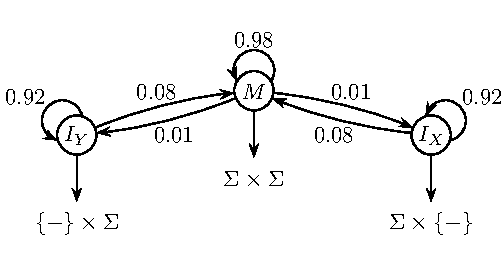
\includegraphics{../figures/simplePairHMM.pdf}
%\end{center}
%\caption[Example of pair hidden Markov model.]{
%State $M$ generates aligned pairs of residues residues, state $I_X$ ($I_Y$) generates
%symbol only in the first (second) sequence.
%}\label{FIGURE:EXAMPLEPAIRHMM}
%\end{figure}
%\section{Use of Pair Hidden Markov Models}\label{SECTION:SIMPLEPHMM}


%We can divide states of pHMM into three types.  Ones that generates symbol in
%both sequences (match states), states that generates symbol in only one sequence
%(indel states) and silent
%states. If pHMM generates  symbols in both sequences we consider those symbols
%to be homologous. We will consider symbols that were not generated by such state
%as indels. Alternative view is to imagine that indel states generate symbol in
%one sequence and gap symbol in the second sequence. In such view pHMM generates
%an alignment.

%Now we show classical pHMM for sequence alignment. It is equivalent to scoring
%scheme of Needleman-Wunsch algorithm with affine gap model. It consists of three
%states: one that generates aligned pairs, and two states for generating
%indels (one for each sequence). Model is shown in figure \ref{FIGURE:SIMPLEPHMM}. 
%
\begin{figure}
\begin{center}
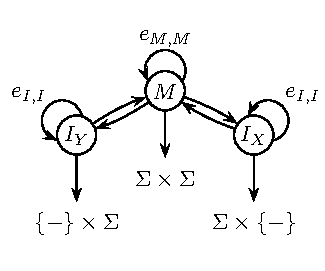
\includegraphics{../figures/pairHMM.pdf}
\end{center}
\caption[Simple pair HMM model for alignment]{Pair hidden Markov model for
pairwise alignment. It has two transitions
parameters $e_{M,M}$ and $e_{I,I}$, since we set $e_{I,M} = 1 - e_{I,I}$ and
$e_{M,I}=\frac12-\frac12e_{M,M}$. Match state $M$ generates aligned pair of symbols
and states $I_X$ and $I_Y$ generates symbols only in $X$ or $Y$ respectively.
Initial distribution is uniform.
}\label{FIGURE:SIMPLEPHMM}
\end{figure}

%As mentioned before, score of the alignment is the probability of state path
%that correspond to such alignment. Therefore we can find the alignment with
%highest score by two dimensional version of Viterbi algorithm. Advantage of
%using this model instead of the Needleman-Wunsch algorithm is that pHMM gives
%probabilistic explanation of the alignments. 



\end{example}

\begin{definition}
Let $H=(\Sigma,V,I,d,e,a)$ be  a pHMM, $X$ and $Y$ be arbitrary sequences over
$\Sigma$ and $\pi$ be a state path. The probability that sequences $X$ and $Y$
were generated by a model $H$  with state path $\pi$ is
\begin{equation}
\Pr\left(X,Y,\pi\mid H\right)=
I_{\pi_0}
\left(
	\prod_{i=1}^{|\pi|}a_{\pi_{i-1},\pi_i}
\right)
\left(
	\prod_{i=0}^{|\pi|}e_{\pi_i,(X[D^x_{i-1}:D^x_{i}],Y[D^y_{i-1}:D^y_{i}])}
\right)
\end{equation}
If $D^x_{|\pi|-1}\not=|X|$ or $D^y_{|\pi|-1}\not=|Y|$ then
$\Pr\left(X,Y,\pi\mid H\right)=0$. 
\end{definition}

Similarly as for HMMs, we can define the probability that sequences $X$ and $Y$ were
generated by the model $H$.

\begin{definition}
Let $H=(\Sigma,V,I,e,a)$ be a pHMM and  $X$ and $Y$ be arbitrary sequences over
$\Sigma$. Then probability that sequences $X$ and $Y$ were generated together by
model $H$ is 
\begin{equation}
\Pr\left(X,Y\mid H\right)=\sum_{\pi}\Pr\left(X,Y,\pi\mid H\right)
\end{equation}
\end{definition}


\subsection{Viterbi algorithm for pair HMM}
\label{SECTION:PAIRHMMVITERBI}
Algorithms operating over pHMMs are similar to those for the regular HMMs, but in
general they have higher computational complexity because over model states with
sequence alignment.
In this section, we describe two-dimensional version of the Viterbi algorithm,
other algorithms are analogous.

The Viterbi algorithm for HMMs computes variables $V[i,v]$ and $B[i,v]$. Every
variable is parametrized by a position in the sequence and a state. For
two-dimensional version, we will add position in the second sequence.

Let $V[i,j,v]$ be the probability of the most probable state path that generated
$X[:i+1]$ and $Y[:j+1]$ and ended in state $v$. Clearly, $\max_{v\in
V}V[|X|-1,|Y|-1,v]$ is the probability of the most probable state path that
generated $X$ and $Y$. Let $B[i,j,v]$ be the last but one state of the most
probable state path that generated $X[:i+1]$ and $Y[:j+1]$ and ended in state
$v$. To make it easier we expect that all states but one are not silent -- they emit
symbol in at least one sequence. The one silent state $s$ (start state) will have $I_s=1$.
 Let $n=|X|$ and $m=|Y|$.


\begin{align}
V[-1,-1,s] &= 1\\
V[-2,i,v] &= V[j,-2,v] = 0, \forall v\in V,-1 \leq i < n, -1\leq j < m\\
V[i,j,v] &= \max_{u\in
V}V[i-d^x_{v},j-d^y_v,u]a_{u,v}e_{v,(X[i:i+d^x_v],Y[j:j+d^y_v])}\label{EQUATION:2DVITERBIF}\\
%V[-1,j,v] &= V[i,0,v] = 0 \\
%V[0,0,v] &= I_{v}e_{v,(?,?)} \\
B[i,j,v] &= \arg\max_{u\in
V}V[i-d^x_{v},j-d^y_v,u]a_{u,v}e_{v,(X[i:i+d^x_v],Y[j:j+d^y_v])}\label{EQUATION:2DVITERBIB}
\end{align}

In equations \ref{EQUATION:2DVITERBIF} and \ref{EQUATION:2DVITERBIB} boundaries for $i$ and $j$ are $
-1\leq i< n,-1\leq j< m$ and $i$ or $j$ is greater than $-1$.


By finding the last state $v$ of the most probable state path and back-tracing
from $B[n-1,m-1,v]$ we can reconstruct the most probable state path. Time
complexity of this algorithm is $O(nm|V|^2)$ (or $O(nm(|V|+t)$ where $t$ is the
number of transitions of $H$) and memory requirements are $O(nm|V|)$. However,
we can use various tricks to decrease memory requirements of such algorithms, as
shown in the section \ref{SECTION:ALGORITHMICIMPROVEMENTS}.

\subsection{Generalized Pair HMMs}


A \abbreviation{generalized pair HMM}{GpHMM} (or pair hidden semi-Markov
process) are combination of HMM and GHMM. Every state generates two
duration lengths $d^x$ and $d^y$ from some joint distribution associated with
the current state $d_v(d^x,d^y)$ and after that it generates two strings $x'$
and $y'$ with lengths $d^x$ and $d^y$ according to the joint distribution
$e_{v,(x',y')}$. This probability distribution can by defined for example by
pair hidden Markov model.  As with GHMMs and unlike pHMMs, the state path is not
sufficient to determine which parts of the sequences were generated by which
state, we also need two sequences of durations.

Drawback of GpHMM is increased computational complexity. For example time
complexity of the Viterbi algorithm is $O(nmk^2d^4)$\cite{Meyer2002} where $k$
is the number of states of a pHMM and $d$ is the maximum duration length.
GpHMMs were successfully used for gene-finding
\cite{SLAM2003,Alexanderson2004,Majoros2005,Meyer2002}. More details are given in
the chapter \ref{CHAPTER:PAIRHMM}.



\section{Other Decoding Methods}
In the previous sections we have described two decoding algorithms: the Viterbi algorithm
that finds the most probable state path  and the Posterior decoding that for
every symbol of the sequence assigns the state that generated such symbol with
maximum probability. 
%In following section we show that the Posterior decoding is
%equivalent to maximizing the expected number of correctly predicted states in
%state path.  
We have shown that in some cases these algorithm recover bad
annotation. However, maximizing the most probable annotation is NP-hard and
therefore it is not tractable. Additionally, the most probable annotation does
not necessary have to be the best approximation of the true annotation.

In this section we will describe highest expected gain decoding framework,
describe already discussed algorithm within this framework and show several
other decoding methods developed in recent years.

\subsection{Highest Expected Gain}

\label{SECTION:HEG}

In this section we will describe a framework for studying decoding algorithm in
a more systematic way. This framework was introduced introduced originally for
conditional random fields \cite{Gross2007}.  To use this framework, we need to
define a gain function, which will express similarity (gain) between two
annotations or state paths. The higher the gain, the more similar those two
sequences are. Gain function is domain specific and can penalize the differences
of the domain specific features in the state paths.  Gain function is not a
similarity in the mathematical sense; it does not even have to be symmetric.

Our goal is to find an annotation that is as similar as possible to the correct
annotation. Problem is that we do not know the correct annotation. Our only
assumption is that the input sequence came from the model and therefore we will
treat the correct annotation as a random variable, with probability distribution
defined by the HMM and the observed sequence. We will seek for annotation that
maximizes the highest expected gain \cite{Nanasi2010,Nanasi2010mgr}.

\begin{definition}
Let $H$ be an HMM and $L$ be the set of all annotations. Any function
$f:L\times L\to \mathbb{R}$ is an \firstUseOf{annotation gain function}.

Let $\Pi$ be the set of all state paths. Any function $f:\Pi\times
\Pi\to\mathbb{R}$ is a \firstUseOf{path gain functions}.

\end{definition}

\begin{note}
We will use term gain function instead of annotation/path gain function if it is
clear from the context.

Machine learning literature often uses a related term of loss function
\cite{Lember2010}. Lower loss mean more similar annotations, that is higher gain. Instead
of maximizing the expected gain we can therefore equivalently minimize the expected
loss.
\end{note}

\begin{definition}
Let $H$ be an HMM, $f$ be a gain function, $X$ be a sequence generated by $H$ and
$\Lambda$ be an annotation of $X$. Then the \firstUseOf{expected gain} of annotation
$\Lambda$ is 
\begin{equation}
E_{\Lambda_X\mid X,H}[f(\Lambda_X,\Lambda)] =
\sum_{\Lambda_X}f(\Lambda_X,\Lambda)\Pr\left(\Lambda_X\mid X,H\right)
\end{equation}
Let $\pi$ be a state path. Then the expected gain of state path $\pi$ is 
\begin{equation}
E_{\pi_X\mid X,H}[f(\pi_X,\pi)] =
\sum_{\pi_X}f(\pi_X,\pi)\Pr\left(\pi_X\mid X,H\right)
\end{equation}

\end{definition}


Once we have HMM $H$, gain function $f$ and the observed sequence $X$,
we are trying to find the annotation/state path maximizing the expected gain. 
\begin{equation}
\Lambda = \arg\max_{\Lambda}E_{\Lambda_X\mid
X,H}\left[f\left(\Lambda_x,\Lambda\right)\right]
\end{equation}

We can express the classical decoding algorithms within this framework to show
its universality. We will define two gain functions: $f_A$ which corresponds to
the  
Viterbi algorithm and the most probable annotation problem and $f_p$ which
corresponds to 
the Posterior decoding.

The gain function $f_A$ is simply identity function (definition for state paths
is analogous).
\begin{equation}
f_A(\Lambda,\Lambda') = \begin{cases}
1 & \text{if $\Lambda = \Lambda'$ }\\
0 & \text{if $\Lambda \not=\Lambda'$}
\end{cases}
\end{equation}
For this gain function $E_{\Lambda_X}[f_A(\Lambda_X,\Lambda)]=\prob{\Lambda\mid
X H}$ and this
maximizing expected gain is 
equivalent to the most probable annotation problem. Similarly if we define gain
as the identity function over state paths, we obtain the most probable state
path problem, which can by solved by the Viterbi algorithm.

Therefore for given sequence finding annotation with highest expected gain is
NP-hard if gain function is part of the input. However, for specific gain
functions we can maximize expected gain in polynomial time.

The gain function $f_P$ compares the two annotations of the same length position
by position and assigns score $1$ to every position where they are equal.
\begin{equation}
f_P(\Lambda,\Lambda') = 
\begin{cases}
0 & \text{if $|\Lambda|\not=|\Lambda'|$}\\
\sum_{i=0}^{|\Lambda|-1}\begin{cases}
1 & \text{if $\Lambda_i=\Lambda'_i$}\\
0 & \text{otherwise}
\end{cases}
\end{cases}
\end{equation}

Similarly, we can define gain function $f_P$ for state paths. In such case
maximizing expected gain is equivalent to the Posterior decoding. Highest
expected gain framework give us another interpretation of scoring function of
the Posterior decoding. Let $\Lambda_X$  have same length as $\Lambda$. From
linearity of the expectation we have \[E_{\Lambda_X}[f_P(\Lambda_X,\Lambda)] =
\sum_{i=0}^{|\Lambda|-1}E_{\Lambda_X[i]}[f_P(\Lambda_X[i],\Lambda[i])]\] We say
that the $i$-th label of $\Lambda$ is correctly predicted if
$f_P(\Lambda_X[i],\Lambda[i])=1$ (which is true if $\Lambda_X[i]=\Lambda[i]$). Therefore  by maximizing $f_P$ we search for
an annotation/state path that maximizes the expected number of correctly
predicted labels/states.

\subsection{Maximum Boundary Accuracy Decoding}

\abbreviation{Maximum boundary accuracy decoding}{MBAD} is used in the gene-finder
CONTRAST \cite{Gross2007}. It
was proposed for \abbreviation{conditional random fields}{CRF}, but since CRF
are similar to HMM, we define it in the terms of HMMs.

This decoding method  maximize the weighted difference between the expected
number of true-positive and false-positive coding region boundaries.

\begin{definition}
Let $\Lambda=\Lambda_0\Lambda_1\dots\Lambda_{n-1}$ be an annotation. A boundary of
annotation $\Lambda$ is every position $i$ where $\Lambda_{i-1}\not=\Lambda_i$. 
\end{definition}

Maximum boundary accuracy decoding has one parameter $\gamma$. Let $B_{\Lambda'}$ be the
set of all boundaries in $\Lambda'$. Then MBAD maximizes the following function:
\begin{equation}
f(\Lambda,\Lambda')=\sum_{i\in B_{\Lambda'}}g(\Lambda,\Lambda',i)
\end{equation}
where 
\begin{equation}
g(\Lambda,\Lambda',i)=
\begin{cases}
1 & \text{if $\Lambda_{i-1}=\Lambda'_{i-1}$ and $\Lambda_{i}=\Lambda'_{i}$}\\
-\gamma& \text{otherwise}
\end{cases}
\end{equation}

From the linearity of the expectation we know that
\[E_{\Lambda}[f(\Lambda,\Lambda)']=\sum_{i\in
B_{\Lambda'}}E_{\Lambda}[g(\Lambda,\Lambda',i)]\] We call
$E_{\Lambda}[g(\Lambda,\Lambda',i)]$ the expected gain of boundary $i$.


Algorithm for finding annotation that maximizes expected gain with function $f$
is following. At first we compute the $P^i_{c_1,c_2}$, the probability that correct annotation
has boundary between colors $c_1$ and $c_2$ is at position $i$. This can be
computed by a variant of the Posterior decoding
since 
\[P_{c_1,c_2}^i=\prob{\Lambda_i=c_1,\Lambda_{i+1}=c_2\mid X,H}\]  
  The expected gain of
boundary at position $i$ between colors $c_1,c_2$  is 
\[P^i_{c_1,c_2}-\gamma (1-P^i_{c_1,c_2})\]
We denote this value by  $B^i_{c_1,c_2}$.

After computing values $B^i_{c_1,c_2}$ we construct graph $G=(V,E)$ where
\begin{align*}
V&=\{v^i_{c_1,c_2}\mid 0\leq i<|X|,c_1,c_2\in C\}\cup\{s\}\\
E&=\{(v^i_{c_1,c_2},v^j_{c_2,c_3})\mid 0\leq i<j< |X|, c_1,c_2,c_3\in C
\}\cup\{(s,v^i_{c_1,c_2}\mid 0\leq i< |X|, c_1,c_2\in C\} 
\end{align*}
where $C$ is the set
of labels. Weight of the edge $(u,v^i_{c_1,c_2})$ is $B^i_{c_1,c_2}$ for all $u\in
V$. Each vertex corresponds to the boundary in the annotation and edges
corresponds to the boundaries of the same block of consecutive labels with the same
color.
There is one to one correspondence between annotations of $X$ and paths in
$G$ starting in $s$ (sequence of vertices corresponds to the sequence of
boundaries which uniquely defines an annotation). Moreover weight of every path
is the expected gain of
the corresponding annotation. $G$ is acyclic and therefore we can find such path in
polynomial time. This can be implemented in $O(|X||C|^2+|X|m^2)$ time and memory
where $m$ is the number of states of HMM $H$. More details of implementation
for HMMs can be found in
\cite{Nanasi2010mgr}.

Intuition behind gain function $f$ is following. Like with the Posterior
decoding, we want to maximize the number of correctly predicted boundaries (the
Posterior decoding maximizes the number of correctly predicted states). The
difference is in the $\gamma$. If $\gamma=0$ then almost every possible boundary
have positive gain and therefore the reconstructed annotation will contain many
false-positive boundaries with very small expected gain. Positive $\gamma$ cause
that boundaries with small posterior probability will have negative expected
gain and therefore it is less likely that they appear in the optimal annotation.


\subsection{Highest Expected Reward Decoding}

\abbreviation{Highest Expected Reward Decoding}{HERD} is the extension of maximum
boundary accuracy decoding. We have developed this decoding for prediction of
recombination of HIV virus.  Further details can be found in \cite{Nanasi2010}
and in my Master thesis \cite{Nanasi2010mgr}.


Genome of some viruses (for example HIV or HCV virus) can be divided into
several subtypes. Moreover, it is possible that virus is mosaic
recombination of viruses from different subtypes (we call this virus
recombinant). In the problem of recombination detection we try to decide if
given sequence $X$ is recombinant sequence. If $X$ is recombinant then we want to find
original subtypes of every part of a sequence $X$. Recombinations can be modeled
by jumping HMMs \cite{Schultz2006} which are HMM with topology specific to this domain.
In this application is 
%In the problem of recombination detection in virus genome In the problem of
%recombination detection in virus RNA is usually jumping HMM \cite{}. 
hard to find exact recombination point since annotations with slightly shifted
boundaries has similar probabilities. Therefore we have defined the following gain
function.

\begin{figure}
\begin{center}
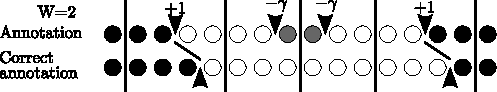
\includegraphics[width=10cm]{../figures/HERDbuddy.pdf}
\end{center}
\caption[Highest Expected Reward Decoding explanation]{
Triangles corresponds to the boundaries. Vertical lines corresponds to the windows
of size $2W$, or smaller to avoid overlaps. Windows around boundaries
represents regions where we search for the corresponding boundaries in the correct
annotation.
The first and the fourth boundary are correctly predicted because in the correct
annotation is boundary between same colors within distance $W=2$.
%correctly predicted (they have penalty $-\gamma$). Because there is no such
%boundary in the correct
%annotation within window.
This picture was taken from \cite{Nanasi2010mgr}.
}\label{FIGURE:HERDBUDDY}
\end{figure}

We say that boundary on position $i$ is correctly predicted, if it satisfy
following conditions.
\begin{enumerate}
\item There is boundary between same labels in the correct annotation on position $j$ and $j$ is
within distance $W$ from $i$ ($|i-j|\leq W$).
\item There is no other boundary between $i$ and $j$. 
\end{enumerate}
Boundaries are illustrated in figure \ref{FIGURE:HERDBUDDY}. 
%In addition, the
%beginning and the end of the sequence are considered to be boundary too (with
%special start and end label).

Let $x$ be the number of correctly
predicted boundaries and $y$ be the number of other boundaries in the proposed
annotation. Then $f(\Lambda,\Lambda')=x-\gamma y$ where $\gamma$ is defined
constant. If $W=1$ then this is equivalent to the Maximum Boundary Accuracy
Decoding. Intuition behind this gain function is that we want to amplify the   
expected gain for the boundary if there are many annotations with similar
boundary.

Optimizing this criteria can be done in $O(|X|W|C||T| + n|C|^2W^2)$ time  and
$O(\sqrt{|X|}|C||V|+W|C||V|+n|C|^2)$ memory. Experimental evaluation,
optimization algorithm and implementation details can be found in
\cite{Nanasi2010,Nanasi2010mgr}.

\subsection{Distance Measures on Annotations}

Another approach to solve similar problem was proposed by {\it Brown,
Truszkowski} in \cite{Brown2010}. Originally their implementation was aimed at
prediction of boundaries in transmembrane proteins \cite{Brown2010}, but later
they successfully adapted their algorithm to jumping HMMs \cite{Truszkowski2011}.
Their approach is trying to solve same problem as HERD: the exact boundaries of
an annotations are hard to find and grouping similar annotation is useful.
At first we give few definitions.

\begin{definition}
Let $d$ be any distance measure defined on annotations. Ball of radius $r$
around annotation $\Lambda$ is 
\begin{equation*}
B_d(\Lambda,r) = \{\Lambda'\mid d(\Lambda,\Lambda')\leq r\}
\end{equation*}
\end{definition}

\begin{definition}
Let $\Lambda=\Lambda_0\Lambda_1\dots\Lambda_{n-1}$ be an annotations. Footprint
of $\Lambda$ is maximal subsequence of $\Lambda$ that does not contain two
identical 
consecutive labels.
\end{definition}

\begin{definition}
Let $b_i(\Lambda)$ be $i$-th boundary of $\Lambda$ and $b(\Lambda)$ be the
number of boundaries in $\Lambda$.
Border shift distance $d_{b}$ is 
\begin{equation*}
d_{b}(\Lambda,\Lambda') = \begin{cases}
\infty & \text{if $\Lambda$ and $\Lambda'$ have different footprint}\\
\max_{i=0}^{b(\Lambda)-1} d_i(\Lambda)-d_i(\Lambda') & \text{otherwise}
\end{cases}
\end{equation*}
and border shift sum distance $d_s$ is 
\begin{equation*}
d_{s}(\Lambda,\Lambda') = \begin{cases}
\infty & \text{if $\Lambda$ and $\Lambda'$ have different footprint}\\
\sum_{i=0}^{b(\Lambda)-1} d_i(\Lambda)-d_i(\Lambda') & \text{otherwise}
\end{cases}
\end{equation*}

\end{definition}

To predict the recombinations of sequences or the annotations of the
transmembrane proteins {\it Brown,
Truszkowski} maximize following function
\begin{equation*}
f_d(\Lambda,\Lambda') = 
\begin{cases}
1 & {\text if }\Lambda\in B_d(\Lambda',r)\\
0 & \text{otherwise}
\end{cases}
\end{equation*}

As distance $d$, they have considered Hamming distance, Border shift distance
and Border shift sum distance \cite{Brown2010}.  If we set $r=0$ then $f_d$ is
same as $f_A$ and therefore finding annotation that maximize $f_d$ is NP-hard.

Maximizing $f_d$ is NP-hard but finding the  annotation with footprint $F$ and
maximal expected gain can be done in polynomial time \cite{Brown2010}. Therefore
{\it Brown and Truszkowski} used following heuristic algorithm: At first they
sample the state path to get footprint with high probability then they used the
polynomial algorithm for finding the annotation with the highest expected gain.

Gain function $f_d$ is similar to $f_A$: the annotation is considered correct if
it is same/very similar to th correct one. However, MBAD and HERD and the
Posterior decoding do not care about overall structure of annotation, they
construct annotation from highly probable ``features''. In contrast to the
decoding function of the HERD, decoding function $f_d$ take in to account
overall structure of the sequence.


\section{Algorithmic Improvements}
\label{SECTION:ALGORITHMICIMPROVEMENTS}

In this section we review implementation details and several algorithmic
improvements of the Viterbi algorithm and the Posterior decoding for HMMs and
pHMMs. Mostly we will assume that HMMs does not have silent states.  Most of these
techniques are easily adjustable to HMMs with silent states. 

\subsection{Basic Implementations}

Implementation of the Viterbi algorithm and the Forward-Backward algorithm can be
done by a two-dimensional dynamic programming, similarly as with the sequence
alignment. Let $H$ be an HMM, $V[i,v]$ be  $n\times m$ matrix where $n$ is the
length of the sequence and $m$ is the number of states of the HMM. $V$ will be the
dynamic programming matrix for the Viterbi algorithm or the Forward algorithm.

Code for the Viterbi algorithm is following:
\begin{lstlisting}
Initialize D[0,*]
for i = 1...n-1:
  for v = 0...m-1:
    V[i,v] = max    [u=0...m-1] V[i-1,u]*[v,X[i]]*a[u,v]
    B[i,v] = argmax [u=0...m-1] V[i-1,u]*[v,X[i]]*a[u,v]
statePath[n-1] = argmax [u=0...m-1] V[n-1,u]
for i=n-1...1:
    statePath[i-1] = B[i,statePath[i]]
\end{lstlisting}

This algorithm runs in $O(nm^2)$ and requires $O(nm)$ memory. Note that values
of row $V[i,\cdot]$ and $B[i,\cdot]$ are computed from rows $V[i-1,\cdot]$ so if
we want just the probability of the most probable state path, we need to
remember only last two rows of $V$ (and we do not need $B$) so the memory
requirements will be $O(n+m)$. If we replace on line $4$ maximum with summation
and remove lines $5-8$, we will obtain the Forward algorithm. Lines $6-8$
implements back-tracing procedure, which will be omitted in the Forward
algorithm. The Backward algorithm is analogous to the Forward algorithm.

Note that if $a[u,v]$ is zero, then value on the right side of lines $4$ nd $5$
is zero. Therefore we have to iterate only for such $u$, that $u\to v$ is
transition in $H$. By this we will reduce time complexity to $O(n(m+t))$ where
$t$ is the number of transitions of $H$ not only for the Viterbi algorithm, but
also for the Forward algorithm and the Posterior decoding.


\subsection{Checkpointing}
\label{SECTION:HMMCHECKPOINTING}
Checkpointing can be used to decrease memory complexity of the Viterbi
algorithm with back-tracing procedure and the Posterior decoding to $O(\sqrt n
m)$.  Similarly, this technique can be used to reduce memory complexity of the
algorithms for pHMMs to $O(nm\sqrt n )$ where $n$ is the length of the longer
sequences and $m$ is the number of states of HMM.

\subsubsection{The Viterbi Algorithm}
While back-tracing, we need access to values of matrix $B$ in decreasing order.
We need only matrix $B$ and last row of $F$. From $i$-th row of $F$ we can
recompute $i+1$-th row of $B$. Therefore we will remember every $k$-th row
of $V$ from which we will recompute blocks of matrix $B$. $B$ will be split into
blocks
$B_0=B[1:k+1,:],B_1=[k+1:2k+2,:],\dots,B_i=B[ik+1:{i+1}k+1,:],\dots$
We will keep in the memory exactly one block of $B$. If we need row that is in block
$B_i$ but $B_i$ is not in memory, we discard current block and compute block
$B_i$ from $V[ik,\cdot]$. Since we need rows of $B$ in decreasing order, we
recompute every block exactly once. If $k=\theta(\sqrt n)$ then the memory
complexity is  $O(n+m\sqrt n)$.

For two dimensional version we keep every $k$-th matrix $V[ik,\cdot,\cdot]$.
Algorithm is analogous to one-dimensional version or to the checkpointing
technique for the Needleman-Wunsch algorithm

\subsubsection{The Posterior Decoding}

In the Posterior decoding need to interlace computations of $F[i,v]$ and
$B[i,v]$ to compute $F[i,v]\cdot B[i,v]$ for all $0\leq i<n,v\in V$. We will
compute $F$ using the checkpointing technique (we compute every $k$-th row of
$F$ and keep in memory only one block).  $B[i,v]$ will be computed row by row
with the version of the  Backward algorithm that need only $O(m)$ memory. When
we compute $B[i,v]$ we compute $F[i,v]$ by checkpointing technique (if $i$ is in
current block then return $F[i,v]$ from current block. Otherwise discard current
block and recompute the block for row $i$). With this approach we can
compute the posterior values with the $O(m\sqrt n)$ memory. We recompute every row at most
once and therefore time complexity will not change.


\subsection{Using Sequence Repetition}

This techniques uses dictionary based encoding schemes to speedup calculation of
algorithms. We will show how to use this technique to Forward algorithm. Details
about how to use this technique to other algorithms can be found in
\cite{Lifshits2009}.


Idea of this speedup is that we reformulate Forward algorithm into sequence of
matrix multiplications.
Let $H=(\Sigma,V,I,e,a)$ be a HMM, $|V|=m$.  Let $M_x[u,v]=a_{u,v}e_{v,x},
u,v\in V,x\in \Sigma$ be the $m\times m$ matrix and $I_x[u]=I_ue_{u,x}$ be
$1\times m$ vector. Matrix $M_x[u,v]$ corresponds to the transition from the
state $u$ to the state $v$ with emission of $x$ from the state $v$.

\begin{lemma}\label{LEMA:MATRIXMULTI}
Let $X=X_1\dots X_n$ be a sequence, $H$ a HMM and $M_x$ and $I_x$ defined as above and
$F[i,\cdot]$ be row vector from forward
Then
\begin{align}
F[0,\cdot] &= I_{X_0}\\
F[i,\cdot] &= I_{X_0}\prod_{j=1}^i M_{X_j}
\end{align}
for all $i< n$.
\end{lemma}

\begin{proof}
We prove this lemma by induction.  If $|X|=1$ then
$F[0,v]=I_{X_0}[v]=I_{v}e_{v,X[0]}$ for all $v\in V$.  Assume that for
$F[k,:] = I_{X_0}\prod_{j=1}^k M_{X_j}$ (note that the  product of zero matrices
is the identity matrix). We have 
\begin{align*}
\left(I_{X_0}\prod_{j=1}^{k+1} M_{X_j}\right)[v] &= 
\left(F[k,:] M_{X_{k+1}}\right)[v]\\ &= \sum_{u\in V} F[k,u]
M_{X_{k+1}}[u,v]\\ &= \sum_{u\in V} F[k,u] a_{u,v}e_{v,X_{k+1} } \\&= F[k+1,v] 
\end{align*}
for all $v$. 
\end{proof}

Consequence is that we can write the Forward algorithm as the sequence of
multiplications of $|\Sigma|$ different matrices. Since matrix multiplication
is associative, we can use repetitive patters to speedup calculation. 
Let $x$ be subsequence of $X$ that has $k>1$ non-overlapping occurrences in $X$.
We can compute $M_{x[0]}M_{x[1]}\dots M_{x[{|x|-1}]}$ once and use it several
times. Let $M_{x}=\prod_{i=0}^{|x|-1}M_{x[i]}$ for any string $x$.

By proper choosing of substrings $x$ we can speedup computation of the Viterbi
algorithm\footnote{For the Viterbi algorithm we need different matrix
multiplication}, the Forward algorithm  or the
Forward-Backward algorithm. Algorithms has following structure:
\begin{enumerate}
\item We choose the \firstUseOf{dictionary} $D$. $D$ is set of string over
alpha bet $\Sigma$. String is a
\firstUseOf{good} if it belongs to $D$.
\item We compute $M_x$ for all $x\in D$.
\item We split input sequence $X[1:]$ into the sequences of good words
$x_0,x_1,\dots,x_{k-1}$ such that $x_0x_1\dots x_{k-1}=X[1:]$.
%and $x_i\in D$ for
%all $0\leq i<k$
\item We compute $I^{X_0}\prod_{i=0}^{k-1}M_{x_i}$ in $O(kf(m))$ time where
$f(m)$ is time needed to compute multiplication of two matrices of size $m\times m$
\end{enumerate}

Lifshits {\it et al.} \cite{Lifshits2009} showed several ways how to choose set
$D$ and split $X$ into sequence of good words. One of them is to use LZ78 factorization
to split $X$ into $O(n/\log n)$ good words. Computation of $M_x$ for all $x\in
D$ can be done in $O(|D|m^3)$. For all $x\in D$, the matrix $M_x$ can be computed in $O(m^3)$
time with following algorithm: if $|x|=1$ then $M_x$ we compute $M_x$ trivially.
If $|x|>1$ then there is $x'\in D$ such that $x=x'a,a\in \Sigma$ and therefore $M_x =
M_{x'}M_{a}$. Since $|D|=O(n/log n)$, computing $M_x$ takes $\Omega(nm^3/log m)$
time if
we use $O(m^3)$ algorithm for computing matrix multiplication. Computing fourth
step of the algorithm takes also $\Omega(nm^3/\log n)$ time and therefore overall time complexity
is $\Omega(nm^3/\log n)$ and that means $\Omega(\log n/m)$ speedup over the
classical implementation of the Forward algorithm for the dense matrices.

It is possible to use different encoding methods. Speedup for the run length encoding 
is $\Omega(r/\log r)$, for the straight-line programs $\Omega(r/m)$ and for the
byte pair encoding $\Omega(r)$ where $r$ is the compression ratio under each
compression scheme. We will not discuss details of this implementations, they
can be found in \cite{Lifshits2009}.

To adapt this approach to the Viterbi algorithm we have to make two adjustments. 
We have to use the max-time matrix multiplication instead of matrix multiplication
\cite{Lifshits2009}. The max-time matrix multiplication is the  matrix multiplication
where summation is replaced with the maximization:
\[M_1\odot M_2 [u,v] = \max_{0\leq i\leq m-1}M_1[u,i]M_2[i,v] \]
where $M_1$ and $M_2$ are matrices of size $m\times m$. This matrix
multiplication is also associative \cite{Lifshits2009}.

The second adaptation is that we have to had ability to reconstruct 
the most probable state path.
After computing $I^{X_0}\prod_{i=0}^{k-1}M_{x_i}$ we do the back-trace to obtain 
the partial state path $\pi'_0,\pi'_1,\dots \pi'_{k}$ which is subsequence of the
most probable state path. Each $\pi'_i$ is state corresponding to the last
sequence of $x_i$. We have to reconstruct state path between $\pi'_i$s; for
every $x_i$ we have to reconstruct state path between $\pi'_{i-1}$ and $\pi'_i$.

All mentioned compression schemes has property,
that for every good string $x$ there are also two good strings $x^1,x^2$ such
that $x=x^1x^2$. To recover state path for every good string $x$ and $u,v\in V$
we have to pre-compute \[R_x[u,v] = \arg\max_{i\in V}M_{x^1}[u,i]M_{x^2}[i,v]\]

Let $x=x_i$. Then $R_{x}[\pi'_{i-1},\pi'_{i}]$ corresponds to the state in the
position of the last symbol of $x^1$. By recursive applying this rule to $x^1$
and $x^2$ we can reconstruct the most probable state path on $x$. By doing this
we can reconstruct it the most probable state path in $O(n)$ time.

Lifshits {\it et al.} applied this  speedup also to the Posterior decoding and
the Baum-Welsch training. 

%Let $X$ be the most probable state path that uses 
%To adapt
%this approach to the Viterbi algorithm we have to use in matrix multiplication
%maximum instead of summation (such multiplication is also associative)
%\cite{Lifshits2009}.

\subsection{On-line Viterbi Algorithm}
\label{SECTION:ONLINEVITERBI}

The On-line Viterbi algorithm is different approach to reduce memory complexity of
the Viterbi algorithm. In this approach we represent matrix $B$ in sparse way
and we keep only those parts of $B$ that can be necessary for reconstruction of
the most probable state path.
We can represent $B$ as the forest $G=(V',E)$ where
\begin{align*}
V' &= \left\{ (i,v)\mid 0\leq i< n, v\in V  \right\}\\
E &= \left\{ (i,v)\to (i-1,B[i,v])\mid 0<i<n,v\in V\right\}
\end{align*}
Edges in this forest are oriented from the children to parents. Roots of the
trees are vertices $(0,v),v\in V$.  Most probable state path that generated
$X[:i]$ and ending in vertex $v$ corresponds to the path from vertex $(i-1,v)$
to root of its tree. Let $S_{i,v}$ be the set of all vertices on the path from
the vertex
$(i,v)$ to the root of its tree. Let $S_i=\cup_{v\in V}S_{i,v}$.
After computation of $B[i,v]$, only the vertices in $S_i$ can be in the most
probable state path so other can be removed. State paths corresponding to
$S_{i,v}$ may be overlap, so by removing others we can reduce memory
requirements.

{\v S}r{\'a}mek {\it et al.} developed data structure that maintains $S_i$
without introducing significant overhead.  Let $G_i$ be the induced subgraph of $G$
consisting from the vertex set $S_i$. Leaf $(j,v)$ is \firstUseOf{unreachable} if
$j<i$.  $G_i$ does not contain unreachable leaf and therefore $G_i$ contains $m$
leaves $(i,v),v\in V$. Construction of $G_{i+1}$ is following.
After computing $B[i+1,\cdot]$ we add vertices $(i+1,v),v\in V$ and edges 
$(i+1,v)\to (i,B[i+1,v]),v\in V$. Vertices $(i+1,v),v\in V$ are the new leaves.
While in $G_{i+1}$ are some internal leaves, we remove them.
After removing all internal leaves, $G_{i+1}$ contains only vertices from $S_i$.
To make $G_i$ smaller, we use the compressed representation of the trees. We compress
chains of vertices with one children into one edge (but we keep
corresponding state path of compressed chain). If we do so, every vertex will
have at most two children and therefore there will be at most $m-1$ internal
nodes. $G_i$ has therefore always $O(m)$ leaves and updating can be done in
$O(m)$ time. Therefore this technique does not alter the asymptotic running time
of the Viterbi algorithm. In practice this technique increased running time by
$5$\% \cite{Sramek2007}.

Improvement in memory requirements can be significant. Even when there exists
HMMs on which this technique will not improve memory requirements
\cite{Sramek2007}, {\v S}r{\'a}mek {\it et al.} reports polylogarithmic 
memory requirements for HMM used for gene finding.
They also proved that for two
state HMMs (with one exception), expected memory complexity of this algorithm is
$O(H\log n)$ where $H$ is constant specific for HMM. Estimation of expected time
complexity for given HMM is still open problem.

Keibler {\it et al. (2007)} developed similar algorithm called the Treeterbi. Both
algorithms are similar, but the Treeterbi does not use the compressed version of the
graph. Both algorithms can be extended to the GHMM and pHMM, the extensions of
the Treeterbi algorithm can found in \cite{Keibler2007}.
